% Global document settings
\documentclass[10pt]{article}

% Packages
\usepackage{tgtermes}
\usepackage{graphicx}
\usepackage{natbib}
\usepackage{authblk}
\usepackage{array}
\usepackage{colortbl}
\usepackage{tocloft}
\usepackage{xcolor}
\usepackage{siunitx}
\usepackage{setspace}
\usepackage{listings}
\usepackage{caption}
\usepackage[T1]{fontenc}
\usepackage[nottoc]{tocbibind}
\usepackage[breaklinks]{hyperref}
\usepackage[font=small,skip=7pt]{caption}

% Custom colours
\definecolor{codegreen}{rgb}{0,0.6,0}
\definecolor{codegray}{rgb}{0.5,0.5,0.5}
\definecolor{codepurple}{rgb}{0.58,0,0.82}
\definecolor{backcolour}{rgb}{0.95,0.95,0.92}

% Listing styles
\lstdefinestyle{mystyle}{
  backgroundcolor=\color{backcolour},
  commentstyle=\color{codegreen},
  keywordstyle=\color{purple},
  numberstyle=\tiny\color{codegray},
  stringstyle=\color{codepurple},
  basicstyle=\ttfamily\footnotesize,
  breakatwhitespace=false,
  breaklines=true,
  captionpos=b,
  keepspaces=true,
  numbers=left,
  numbersep=5pt,
  showspaces=false,
  showstringspaces=true,
  showtabs=false,
  tabsize=2
  }
  \lstset{style=mystyle}

  % Custom commands
  \renewcommand{\bibname}{References} % Change bibliography title
  \renewcommand\cftsecafterpnum{\vskip8pt}
  \renewcommand{\lstlistlistingname}{List of \lstlistingname s}
  \renewcommand{\bibsection}{\section*{Bibliography}}
  \renewcommand{\contentsname}{Table of Contents}
  \renewcommand{\bibsection}{\section{\bibname}}
  \renewcommand{\cftsecleader}{\cftdotfill{\cftdotsep}}

  % Custom settings
  \captionsetup{justification=centering}
  \PassOptionsToPackage{hyphens}{url}
  \urlstyle{same}
  \def\Urlmuskip{0mu}
  \def\UrlBreaks{\do\/\do-}
  \hypersetup{
    colorlinks = true,
    urlcolor = blue,
    linkcolor = black,
    citecolor = black,
  breaklinks=true,
  pdfpagemode=UseOutlines,
  bookmarksopen=true,
  bookmarksopenlevel=2,
  bookmarksnumbered=true
  }

  \title{\textbf{Comparative Analysis of Structural and Functional Neuroimaging in Alzheimer’s Disease: }A Hypothetical Multi-Modal Approach}
  \author[ ]{K23003985}
  % \affil[ ]{\textbf{King’s College London}}
  % \affil[ ]{\href{mailto:public@danielburger.online}{public@danielburger.online}}
  \date{\textit{5. December 2023}}

\begin{document}
% \pagenumbering{roman}
% \counterwithin{lstlisting}{section}
% \counterwithin{figure}{section}
% \counterwithin{table}{section}

\maketitle
% \thispagestyle{empty}

% Double spacing for feedback
\doublespacing

\begin{sloppypar} % For better line breaks
  %   \begin{abstract}
  %     To be created.
  %   \end{abstract}
  %   \pagebreak

  % \pagenumbering{Roman}
  % \tableofcontents
  % \pagebreak

  % \listoffigures
  % \pagebreak

  % \listoftables
  % \pagebreak

  % Back to normal numbering
  \pagenumbering{arabic}

  \section{Introduction}
  \label{sec:introduction}

  Neurodegenerative research, particularly in Alzheimer’s disease (AD), presents significant challenges due to its gradual onset and cognitive decline. This essay aims to explore a hypothetical study design using a multi-modal neuroimaging approach to uncover changes in AD, with a specific focus on beta-amyloid plaques and tau protein tangles. These are critical neuropathological markers known for their pivotal role in the disease’s progression and its clinical manifestations, such as memory loss and cognitive impairment \citep{heneka_neuroinflammation_2015,marttinen_molecular_2018}. The primary objective of this hypothetical study is to critically evaluate the capabilities and limitations of various neuroimaging modalities, notably positron emission tomography (PET) and magnetic resonance imaging (MRI), in detecting these biomarkers. It is important to note the current debate in the scientific community regarding the sequence and interrelation of these biomarkers, particularly how neurodegeneration may relate to amyloid-beta deposition \citep{besson_cognitive_2015}. This understanding is crucial for influencing future research and clinical approaches in AD.

  Grounded in the hypothesis that specific imaging biomarkers are associated with the pathophysiology of AD, this hypothetical study endeavours to draw a more direct connection between these biomarkers and the clinical symptoms of AD. PET, with its ability to visualise metabolic processes, and MRI, known for its high spatial resolution, are anticipated to offer unique insights into the accumulation and impact of beta-amyloid plaques and tau tangles. The proposed multi-modal imaging approach is expected to advance our understanding of AD, potentially leading to earlier diagnosis and improved therapeutic strategies.

  \section{Understanding Alzheimer’s Disease}
  \label{sec:alzheimers-disease}

  AD is a complex neurodegenerative disorder characterised by a range of neuropathological changes and clinical manifestations. Central to its pathology are extracellular aggregated amyloid fibrils and plaques, mainly composed of fibrillary $A\beta$ peptide, and intracellular neurofibrillary tangles (NFTs), mainly built up of hyperphosphorylated tau protein, leading to dysfunction and loss of synapses and contributing to cognitive decline and disruption of neuronal networks \citep{heneka_neuroinflammation_2015,cai_magnetic_2020}.

  Recent advances have shed light on the molecular mechanisms underpinning these processes, highlighting the critical impact of synaptotoxicity and neuroinflammation on AD progression. Neuroinflammation, involving the activation of microglia and astrocytes, has been increasingly recognised for its role in exacerbating AD pathology. PET imaging studies, such as those by \cite{zhou_pet_2021}, have revealed the coexistence of amyloid deposition, neurofibrillary tangles, and neuroinflammation in AD brains, offering new insights into disease mechanisms and potential imaging biomarkers. PET imaging studies have been pivotal in visualising the interplay of amyloid deposition, neurofibrillary tangles, and neuroinflammation in the brains of AD patients. \autoref{fig:pib-ratio} provides a visual representation of the baseline global cortical PIB ratios and baseline ventricular volumes across different clinical groups, underscoring the neuroimaging changes associated with Alzheimer’s disease \citep{jack_serial_2009}. This evidence supports the notion that specific imaging biomarkers, detectable through techniques like PET, are intimately linked with the underlying pathophysiology of AD.

  \begin{figure}[ht]
    \centering
    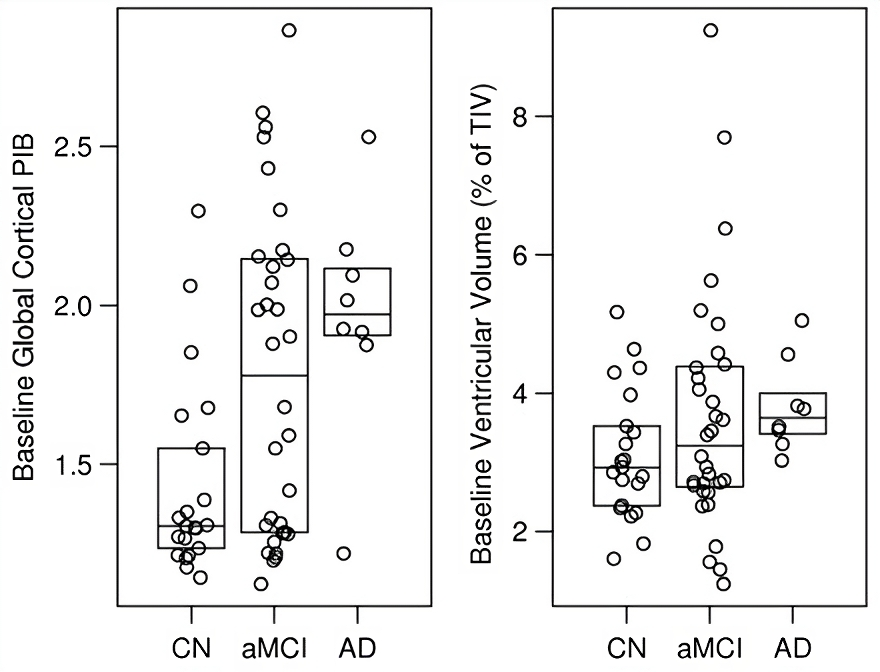
\includegraphics[width=\textwidth]{figures/pib-ratio.png}
    \caption[Baseline global cortical Pittsburgh Compound B (PIB) ratio and baseline ventricular volume by clinical diagnosis in Alzheimer’s Disease.]{\textbf{Baseline global cortical Pittsburgh Compound B (PIB) ratio and baseline ventricular volume by clinical diagnosis in Alzheimer’s Disease.} The figure compares global PIB ratios and ventricular volumes across different clinical groups, highlighting the neuroimaging distinctions characteristic of Alzheimer’s Disease progression. (Adapted from \cite{jack_serial_2009}).}
    \label{fig:pib-ratio}
  \end{figure}

  Synaptic dysfunction in AD, encompassing alterations in neurotransmitter systems and synaptic plasticity, has recently gained attention as a central feature of the disease, often referred to as ‘synaptopathy’. This concept underscores the significance of synaptic impairment in disease progression and its potential as a target for therapeutic interventions \citep{meftah_alzheimers_2023}. The interplay between these neuropathological changes and neuroinflammation is crucial for understanding AD mechanisms and developing new treatments.

  Additionally, rodent models have been instrumental in elucidating the links between neuroinflammation and AD pathology. However, translating these findings to human AD remains challenging, underscoring the need for advanced neuroimaging techniques to bridge this gap. Recent studies emphasise the importance of considering the interplay between neuropathological changes and neuroinflammation when designing neuroimaging studies to investigate structural and functional changes in AD \citep{nazem_rodent_2015}.

  \section{Objectives and Hypotheses of the Study}
  \label{sec:objectives-and-hypotheses}

  The primary objective of this hypothetical study is to explain the structural and functional changes in AD using neuroimaging techniques. Building upon the existing foundation of AD research, this study aims to identify and validate neuroimaging biomarkers that correlate with AD’s neuropathological progression and clinical manifestations. It is key to consider the findings from \cite{besson_cognitive_2015}, which indicate that individuals positive for different biomarkers show varying cognitive and brain profiles. For instance, differences in executive function performance among MRI-positive individuals and distinct patterns of hypometabolism and $A\beta$ deposition in different subgroups highlight the complex interplay of these biomarkers in AD \citep{besson_cognitive_2015}.

  Central to our hypothesis is the belief that certain neuroimaging biomarkers, specifically those related to amyloid-beta plaques, tau protein tangles, and hippocampal volume loss, are intimately linked with the underlying pathophysiology of AD. These biomarkers have been selected for their proven significance in AD neuropathology and their potential to provide detailed insights into disease progression. For instance, PET imaging utilises advanced $A\beta$ tracers like 11C-PIB and 18F-labelled compounds for early detection of amyloid accumulation, crucial in AD’s differential diagnosis and monitoring disease progression from MCI to dementia \citep{bao_pet_2021}. Similarly, MRI’s ability to quantify hippocampal atrophy offers a structural perspective on neurodegeneration \citep{besson_cognitive_2015}.

  Furthermore, this hypothetical study emphasises the role of $A\beta$ PET imaging in differentiating AD from other dementias and predicting the progression from MCI to AD dementia, highlighting its utility in clinical settings. This approach aims to uncover synergistic biomarkers that could offer a more comprehensive view of AD pathology, surpassing the insights provided by single-modality imaging.

  The selection of these biomarkers and neuroimaging techniques is supported by significant evidence, including findings from the Alzheimer’s Disease Neuroimaging Initiative (ADNI). ADNI’s work in identifying and validating neuroimaging biomarkers, such as hippocampal volume loss and amyloid deposition, has been essential in preclinical AD \citep{saykin_genetic_2015}. By integrating these insights with genetic data, the hypothetical study seeks to deepen the understanding of AD pathophysiology and contribute to developing targeted therapeutic interventions.

  \section{Neuroimaging Methods for the Study}
  \label{sec:neuroimaging-methods}

  This hypothetical study will employ PET imaging with amyloid and tau-specific radiotracers and advanced MRI techniques, each chosen for their unique contributions to understanding AD pathology.

  PET imaging is invaluable in visualising and quantifying beta-amyloid plaques and tau tangles, providing direct insights into the molecular pathology of AD \citep{jack_serial_2009}. This method excels in sensitivity and specificity but is limited by its use of ionising radiation and availability in some clinical settings \citep{bao_pet_2021}.

  Conversely, MRI offers detailed anatomical and microstructural information, particularly with advancements in MRI texture analysis. This includes brain volume, cortical thickness, hippocampal atrophy, and changes in image texture due to the deposition of $A\beta$ peptide and NFTs, indicative of neurodegenerative changes in AD \citep{cai_magnetic_2020}. Recent advancements in MRI texture analysis have further enhanced its capacity to detect microstructural alterations associated with AD pathology. While MRI avoids radiation exposure and is ideal for repeated measurements, it may be less sensitive to specific molecular changes than PET imaging.

  The study will leverage multi-modal neuroimaging, integrating PET and MRI data, to provide a holistic view of AD pathology. This approach aims to mitigate the limitations inherent to each modality. By combining PET’s molecular sensitivity with MRI’s structural resolution, we can achieve a more comprehensive understanding of AD, enhancing both the detection and characterisation of neuropathological changes.

  Ethical and practical considerations, including patient comfort and the cost-effectiveness of these techniques, are an essential part of this study design that should be considered. This study seeks to not only advance scientific understanding but also to inform clinical practices in a manner that is both patient-centred and resource-efficient.

  \section{Justification of Study Design}
  \label{sec:justification-of-study-design}

  A vital aspect of the design is the implementation of stringent inclusion and exclusion criteria coupled with advanced statistical methods to control for potential biases and confounding factors.

  Participants will be meticulously selected based on rigorous criteria, including a confirmed AD diagnosis following established guidelines. Exclusion criteria will specifically address comorbid conditions like vascular dementia or medication effects that could obscure neuroimaging results. For instance, individuals with a history of significant head trauma or psychiatric conditions that might affect cognitive function will be excluded. Additionally, demographic variables such as age, sex, and education level will be carefully matched across study groups to address potential confounding effects.

  Advanced statistical techniques, including propensity score matching and multivariate regression models, will be employed to mitigate bias further. These methods will help ensure that observed differences in neuroimaging biomarkers reflect AD pathology and are not skewed by extraneous variables.

  Addressing the limitations inherent in neuroimaging techniques is also a crucial component of the hypothetical study design. Standardised image acquisition and processing protocols will be rigorously applied across all study sites to ensure consistency. Quality control measures, including periodic calibration of equipment and validation of software algorithms, will be implemented to maintain the integrity of the neuroimaging data.

  Ethical considerations, particularly concerning participant consent and data confidentiality, will be strictly adhered to. This adherence to ethical guidelines ensures that the study respects participant rights and upholds the integrity of the research process.

  Finally, the findings’ practical application and potential generalisability will be necessary. The author aims to produce results that advance scientific understanding and have tangible implications for clinical practice and future AD research.

  \section{Conclusion}
  \label{sec:conclusion}

  This study aims to contribute to our understanding of this complex neurodegenerative condition. Despite its promise, the author must acknowledge certain limitations, as these highlight areas for future research and underscore the need for a nuanced understanding of AD pathology.

  One notable limitation is the cross-sectional nature of this study, which limits our ability to infer causal or temporal relationships between neuroimaging biomarkers and AD progression. Longitudinal studies are essential for understanding the dynamic nature of AD, offering insights into how these biomarkers evolve.

  The reliance on neuroimaging biomarkers, while informative, may introduce measurement error and variability. Future studies should integrate these biomarkers with other indicators, such as cerebrospinal fluid markers and genetic profiles, to provide a more comprehensive characterisation of AD pathology.

  Although limited, these insights are invaluable and can be used to develop new diagnostic and therapeutic strategies for AD and other neurodegenerative conditions. The study’s findings can influence clinical practices and guide future research directions.

  Looking ahead, research should focus on incorporating multi-modal biomarkers, conducting longitudinal assessments, and diversifying participant populations. Integrating advanced neuroimaging techniques with genomic and proteomic data promises a more profound understanding of AD mechanisms, paving the way for identifying new intervention targets.

  \pagebreak
  \singlespacing % No need for double spacing in the references
  \bibliographystyle{references/custom-apa}
  \bibliography{references/bibliography}

\end{sloppypar}
\end{document}